\documentclass[a4paper,11pt] {article}
% Default margins are too wide all the way around. I reset them here
\setlength{\topmargin}{.5in}
\setlength{\textheight}{9in}
\setlength{\oddsidemargin}{.125in}
\setlength{\textwidth}{6.25in}

\usepackage{color}
\usepackage[utf8]{inputenc}
\usepackage{graphicx}
\usepackage{float}
\usepackage{pdfpages}
\usepackage{amsthm}
\usepackage{amsmath,amsfonts,amssymb,amsthm}
\theoremstyle{definition}
\newtheorem{defn}{Definition}[section]
\newtheorem{conj}{Conjecture}[section]
\newtheorem{exmp}{Example}[section]

\definecolor{javared}{rgb}{0.6,0,0} % for strings
\definecolor{javagreen}{rgb}{0.25,0.5,0.35} % comments
\definecolor{javapurple}{rgb}{0.5,0,0.35} % keywords
\definecolor{javadocblue}{rgb}{0.25,0.35,0.75} % javadoc
%\usepackage[french]{babel}
\usepackage[T1]{fontenc}


\begin{document}
\title{\textbf{Usability \& Skeuomorphism}}
\author{\textbf{Bodart Xavier} - \textbf{Chapeaux Thomas} - \textbf{Mayeur Bernard} \\
Université Libre de Bruxelles}

\maketitle
\begin{center}

\textbf{INFO-F501 Information technology in society} \\
Luc WILKIN
\end{center}
\begin{center}

~\\


\includegraphics[scale=0.15]{ULBjea.jpg}
\end{center}
\pagebreak
\tableofcontents
\pagebreak
\section{Introduction}

Most tools, from wristwatches and squirt guns to smartphones and industrial softwares, rely on sophisticated technology hidden from the average user.

\section{Theoretical concepts \& design principles}
\subsection{Perceived affordance}
Perceived affordance represents the quality of an object to suggest its utilization. This concept is quite important in object-design due to the fact that it may represents the main source of information about the usage of the object. Indeed, people tends to read less and less the usage notice. In addition, this concept may reinforce the feeling of experience of a person for a given object.
\begin{figure}[h]
\centering
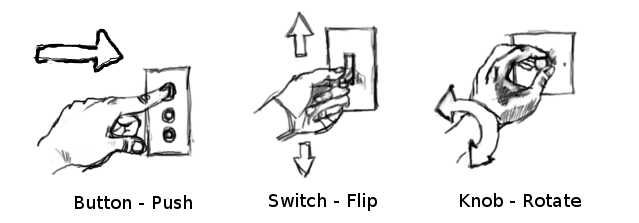
\includegraphics[scale=0.40]{switches-only.png}
\caption{By their forms, buttons,switches or knobs often suggest their working.}
\end{figure}

Perceived affordance is not always the same as real affordance. Indeed, design can rarely explain the complete working of complex objects. The perceived affordance is only capable of showing primitive properties of its usage. Furthermore, a bad design may induce an usage more difficult than the correct design.%http://www.interaction-design.org/encyclopedia/affordances.html
\begin{figure}[h]
\centering
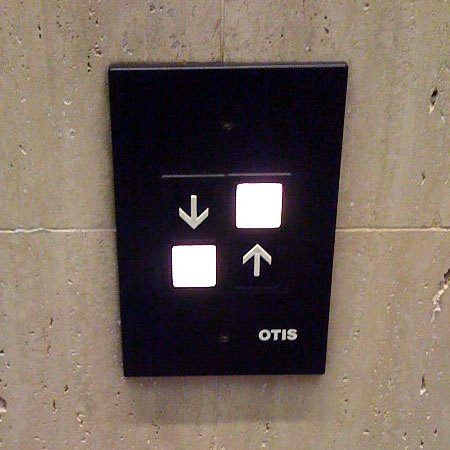
\includegraphics[scale=0.20]{bad-switches.jpg}
\caption{What would you do in front of such a lift panel?}
\end{figure}
\subsection{Natural mapping}
Natural mapping is the concept of organizing controllers in the same arrangement as the objects on which they have an influence to guarantee the expected result. This principle will often lead to an increase in perceived affordance.\\

A common example to illustrate this concept is the placement of the buttons that control the different stoves of your kitchen.It's obvious that the most left-top button will regulate the temperature of the most left-top stove.\\
 \begin{minipage}{\linewidth}
      \centering
      \begin{minipage}{0.45\linewidth}
          \begin{figure}[H]
          \centering
              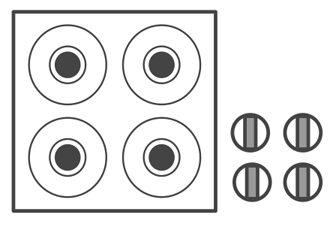
\includegraphics[scale=0.3]{stove_natural.png}
              \caption{Scheme of a four stoves set with their corresponding knobs}
          \end{figure}
      \end{minipage}
      \hspace{0.05\linewidth}
      \begin{minipage}{0.45\linewidth}
          \begin{figure}[H]
                    \centering
              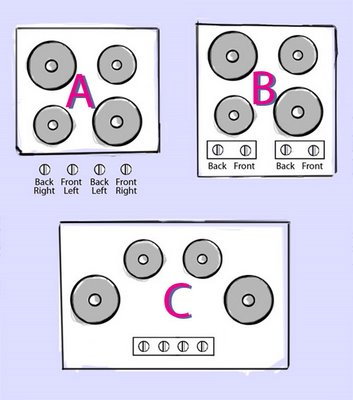
\includegraphics[scale=0.4]{NormanBurners.jpg}
              \caption{These designs work only if you have the same assumption as the designer}
          \end{figure}
      \end{minipage}
  \end{minipage}
  \bigskip


Unfortunately, this principle may sometimes induce extra design cost and may also depends on the point of view of the designer: Even if it seems logical for certain arrangement such stoves or the control of the electronic windows of the car, One can still doubt about the mapping of light switches(\textit{"Does this switch controls  the lights of the front of the room because it is above the others ?"}). %http://karikariboberry.blogspot.be/2008/09/natural-mapping.html
\subsection{Feedback}
\newtheorem{mydef}{Definition}
\begin{mydef}
\textbf{THOMAS} : Je ne comprends pas la fin de cette définition.
\textit{\textbf{Feedback}} is the return of a fraction of the output signal from an amplifier, microphone, or other device to the input of the same device; sound distortion produced by this.%http://www.oxforddictionaries.com/definition/english/feedback
\end{mydef}

In our case, feedback represents any action that could indicate to the user that its interaction with the item was taken into account. In certain cases, feedback can be done implicitly by the quality and the design of the object itself. For example, when a push button is  pressed, one can hear a clicking sound. On the other hand, feedback often requires, in our modern technologies, additional functions like vibrating or emitting sounds that corresponds to states of the device. Theses retro-actions have to provide enough information to the user in order to avoid his frustration about a mistaken usage.
\begin{figure}[h]
\centering
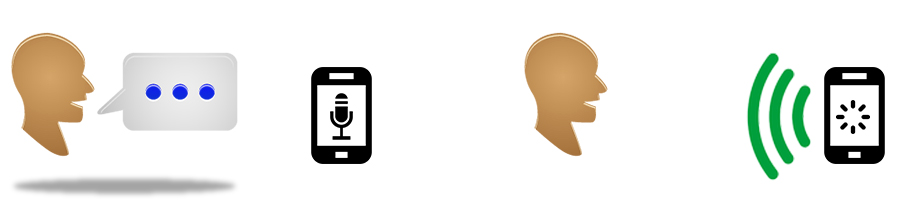
\includegraphics[scale=0.5]{retro-action-speaking.jpg}
\caption{After the user gives a command, the device emits a sound to confirm that it is analyzing the request}
\end{figure}
\subsection{Additional design principles}
As presented in %Source vers l'article...
, one can also add two principles to a good design:
\begin{itemize}
\item \textbf{Provide a good conceptual model}: The idea is to provide a precise information model about the good usage of the item, or the way to maintain it. Written instructions should guarantee the good usage of the item. The design of such scheme is really important and should be extremely clear.
\item \textbf{Make things visible}: Certain of our modern items can be seen as real complex state machines due to the number of actions they can propose. The basic idea behind this principle is to provide a display which shows the current state and the available actions. A good example to this is the usage of a new VoIP telephone which allow a user to start a conference with several other people. Such telephone are often equipped with a large display which can show different contacts number, propose features to start conference or even to place a call on hold in order to answer to another call.
\end{itemize}

 \begin{minipage}{\linewidth}
      \centering
      \begin{minipage}{0.45\linewidth}
          \begin{figure}[H]
          \centering
              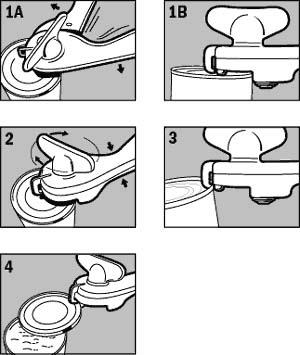
\includegraphics[scale=0.4]{can-opener}
              \caption{Does such model give enough information about the usage of a can-opener ?}
          \end{figure}
      \end{minipage}
      \hspace{0.05\linewidth}
      \begin{minipage}{0.45\linewidth}
          \begin{figure}[H]
                    \centering
              \caption{This void phone has a big display to propose multiple commands}
          \end{figure}
      \end{minipage}
  \end{minipage}

\subsection{Constraints}


\subsubsection{Physical constraints}
\subsubsection{Logical constraints}
\subsubsection{Cultural constraints}
\subsubsection{Semantic constraints}
\subsection{Skeuomorphism}
\subsection{Flat design}

\section{Evolution of the computer-interface}
\subsection{Command line interpreter}
\subsection{Graphical interface \& computer mouse}
\subsection{Touch interface}
\subsection{Voice interface}
\subsection{Neural interface}
\section{Experiment}
\subsection{Definition of the experiment}
\subsection{Results analysis}
\subsection{Comparison with previous studies}
\section{Conclusion}
%Bibliography
\end{document}
